\documentclass[12pt, letterpaper, twoside]{report}
\usepackage[utf8]{inputenc}
\usepackage{graphicx}
\usepackage{verbatim}
\graphicspath{{images/}}
\usepackage{url}

\title{\textbf{autorank}}
\author{Mohammad Sorkhian}
\date{2020 July 31}

\begin{document}

\maketitle

\chapter{Introduction}
\section{What is \textbf{autorank}}
Autorank simplify the comparison between (multiple) paired populations. 
The performance measures on each data set are then the paired samples, 
the difference in the central tendency (e.g., the mean or median) 
can be used to rank the different algorithms.

The goal of Autorank is to simplify the statistical analysis for non-experts. 
Autorank takes care of all of the above with a single function call. 
Additional functions allow the generation of appropriate plots, result tables, 
and even of a complete latex document. All that is required is the data about 
the populations is in a Pandas dataframe.

\section{What is the problem?}
We would like to compare top countries in terms of new detected \textit{Covid-19} cases and 
for better comparison and produce a comprehensive report, we have used this tool.  

\section{Data source}
For this comparison, we have used the \textit{Covid-19} data from WHO and 
have extracted the part of the data that we want to feed the autorank.
\\ \url{https://covid19.who.int/WHO-COVID-19-global-data.csv}

\section{Description of workflow}
\begin{itemize}
  \item Imported pandas, matplotlib.pyplot and autorank libraries.
  \item Downloaded the data with "wget" form the WHO website and read the file into a dataframe.
  \item Grouped the database by "country".
  \item Made a series for each country based on its new \textit{Covid-19} detected cases and converted it into a dataframe.
  \item Extracted top countries based on their total new detected cases.
  \item Used matplotlib to plot the mean value of these top countries and save it.
  \item Used autorank to make an analytical report.
  \item Used autorank built-in functions to plot and print the result.
  \item Used LaTex to creat report PDF.
  \item Created Makefile to automate this procedure.
\end{itemize}

\chapter{Graphs}
\section{autorank Graph}
In this section we see the autorank plot
\begin{figure}[ht]
    \centering
    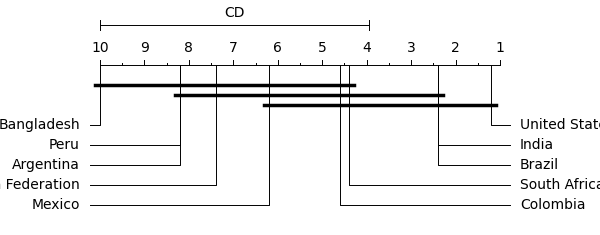
\includegraphics[width=0.8\textwidth]{autorank.png}
    \caption{autorank plot}
    \label{fig:autorank}
\end{figure} 

\section{matplotlib Garaph}
 In this section we see the top countries plot
\begin{figure}[ht]
    \centering
    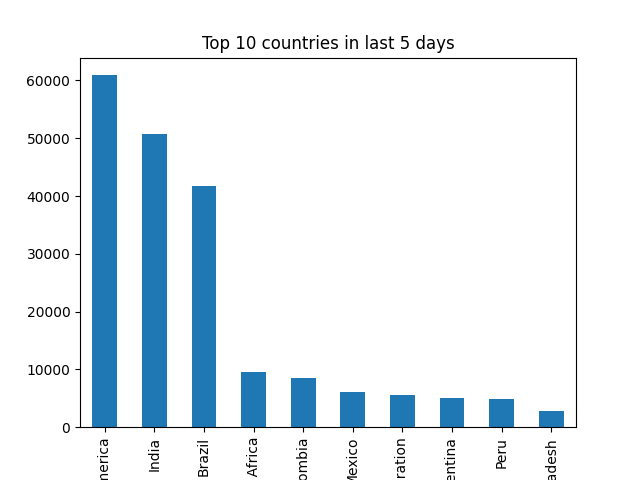
\includegraphics[width=0.8\textwidth]{TopCountries.png}
    \caption{Countries with highest rate of new \textit{Covid-19} detected cases}
    \label{fig:TopCountries}
\end{figure}

\chapter{autorank Reports}
 \verbatiminput{autorankReport.txt}

 \begin{abstract}
  autorank is a simple Python package with one task: simplify the comparison between (multiple) paired populations. This is, for example, required if the performance different machine learning algorithms or simulations should be compared on multiple data sets. The performance measures on each data set are then the paired samples, the difference in the central tendency (e.g., the mean or median) can be used to rank the different algorithms. In \ref{fig:autorank} you can see one output sample of this library
 \end{abstract}
 
@article{Herbold2020,
  doi = {10.21105/joss.02173},
  url = {\url{https://doi.org/10.21105/joss.02173}},
  year = {2020},
  publisher = {The Open Journal},
  volume = {5},
  number = {48},
  pages = {2173},
  author = {Steffen Herbold},
  title = {Autorank: A Python package for 
  automated ranking of classifiers},
  journal = {Journal of Open Source Software}
}

 \end{document}